\section{Building models}
\begin{frame}{Time to assemble pieces!}
\begin{itemize}
\item In Chapter 3, we learned fundamental building blocks.
\item In principle: we can now build neural network based models for MANY problems involving image-like data (2D structured data) and natural language-like data (sequences).
\end{itemize}
\vspace{7mm}
\begin{figure}
  \begin{center}
    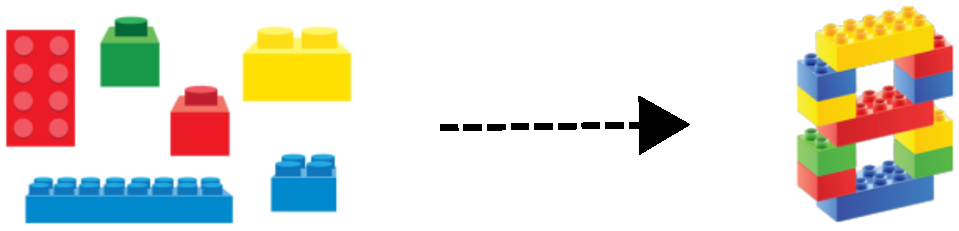
\includegraphics[width=0.6\linewidth]{figures/lego.pdf}
  \end{center}
\end{figure}
\vspace{7mm}
\scriptsize{Figures adapted from \cite{le2020neurocoder} for illustration.}
% \begin{minipage}{0.45\linewidth}
%   \begin{center}
%     \includegraphics[width=0.7\linewidth]{figures/lego_pieces.png}
%   \end{center}
% \end{minipage}
%\begin{minipage}{0.45\linewidth}
%\begin{figure}
%  \begin{center}
%    \includegraphics[width=0.3\linewidth]{figures/lego_asembled.png}
%  \end{center}
%\end{figure}
%\end{minipage}
%\hspace{3mm}
\end{frame}

\begin{frame}{Haven't we already built models?}
\begin{itemize}
\item Yes. For some tasks, building models was straightforward.\\ Example:
\item[-] Basic image classification models (assignment 2): convolutional layers, pooling layers, fully connected layers, output classifier layer (softmax). 
\item[-] Basic language models (assignment 3): recurrent neural networks, input embedding layer, output classification layer.
\item But you can do much more using what we learned in Chapter 3.
\item[-] E.g. sequence to sequence problems.
\end{itemize}
\end{frame}

\begin{frame}{Preliminary comments}
\begin{itemize}
\item We have input(s) and output(s) defined by the task.
\item\textbf{Basic idea}:  We parameterize the input-to-output transformation
as a \textbf{pipeline of multiple neural network layers/blocks}.
\item[-] If each component is differentiable (i.e. we can compute gradients), the whole model can be trained in an \emphbf{end-to-end fashion}.
\item \emphbf{End-to-end differentiable models}: all parameters of the entire model are jointly optimized to minimize a common loss(es).
\item[-] One of the key aspects (advantage/power) of deep learning.
\item[-] E.g. replaced human engineered, hand-crafted input feature engineering. These features were typically not optimized together with the model parameters. Now, it's part of the model.
\end{itemize}
\end{frame}

\begin{frame}{Sequence to sequence problems}
\vspace{-3mm}
Many tasks are of type \emphbf{sequence-to-sequence}:\\
An input sequence has to be transformed into an output sequence.
\vsp
\begin{itemize}
\item Speech recognition: audio speech signals to written texts.
\item Machine translation: source texts to target texts.
\item Some mathematical problem solving (Assignment 4).
\end{itemize}
\vsp
\begin{minipage}{0.45\linewidth}
\begin{figure}
  \begin{center}
    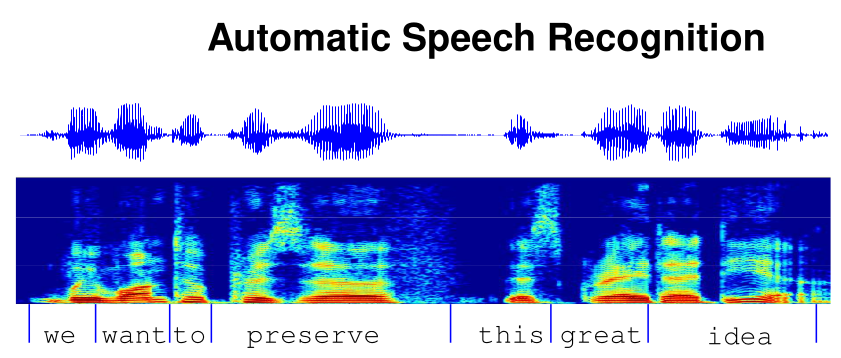
\includegraphics[width=0.9\linewidth]{figures/asr_illu.png}
  \end{center}
\end{figure}
\end{minipage}
%\hspace{3mm}
\begin{minipage}{0.45\linewidth}
\begin{figure}
  \begin{center}
    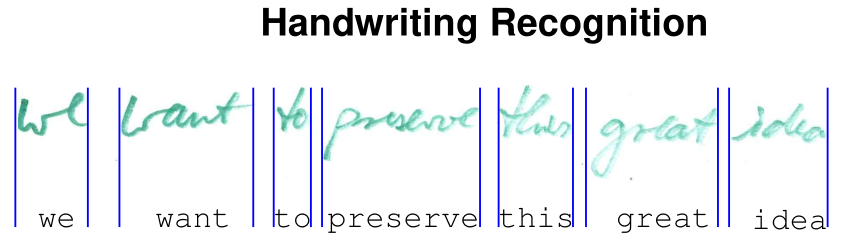
\includegraphics[width=0.9\linewidth]{figures/hw_illu.png}
  \end{center}
\end{figure}
\end{minipage}\\
\vsp
%\hspace{3mm}
 \begin{minipage}{0.45\linewidth}
   \begin{center}
     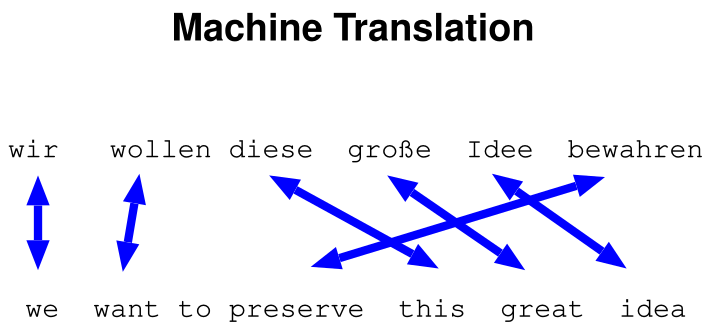
\includegraphics[width=0.9\linewidth]{figures/trans_illu.png}
   \end{center}
 \end{minipage}
\begin{minipage}{0.45\linewidth}
We will be using machine translation as a generic example to illustrate the problem.
 \end{minipage}\\
\vsp
\scriptsize{Figures taken from \cite{neylecture2019}.}
\end{frame}

\begin{frame}{Encoder-Decoder Models}
A generic model to solve sequence-to-sequence problems, w/ 2 RNNs:
\begin{itemize}
\item The first RNN \emphbf{encodes} the input/source sequence.
\item The final encoder-RNN state can be used to initialize the
initial state for the second RNN.
\item The second RNN \emphbf{decodes} the output/target sequence.
\end{itemize}
\begin{figure}
  \begin{center}
    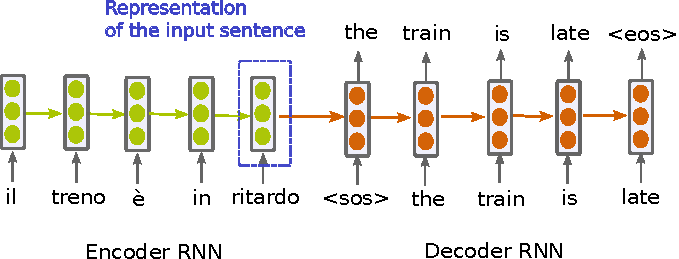
\includegraphics[height=0.5\textheight]{figures/enc-dec.pdf}
  \end{center}
\end{figure}
\end{frame}

\begin{frame}{Encoder-Decoder Models,\\Training}
\textbf{You should feel that training this model is straightforward!}
\begin{itemize}
\item During training, the target sentences are available.
\item The decoder RNN can be trained just as a language model (shifted input/target).
\item Use the cross entropy loss, only from the target sentence
\end{itemize}
\vsp
\pause
\textbf{What about ``decoding"?}
\begin{itemize}
\item At test time, you only have a ``source" sentence available.
\item ... and we want to extract the most likely target sentence according to the model.
\item This is similar to what you are doing in Assignment 3 with language models.
\item ... some extensions to improve decoding is possible.
\end{itemize}
\end{frame}

\begin{frame}{Encoder-Decoder Models,\\ Beam search}
\begin{itemize}
\item We want to find the most likely output sequence accoring to the model.
\item Ideally, we should do exhautive search: evaluate any possible sentences, the sentence with the highest probability is the answer.
\item This is too expensive/impossible!
\item Practical solutions:
\begin{itemize}
\item[-] \emphbf{Greedy search}: take the argmax at each step (like in assignment 3).
\item[-] better: \emphbf{beam search} also known as top-K search.
\end{itemize}
\end{itemize}
\end{frame}

\begin{frame}{Encoder-Decoder Models,\\ Beam search, illustration}
\begin{figure}
  \begin{center}
    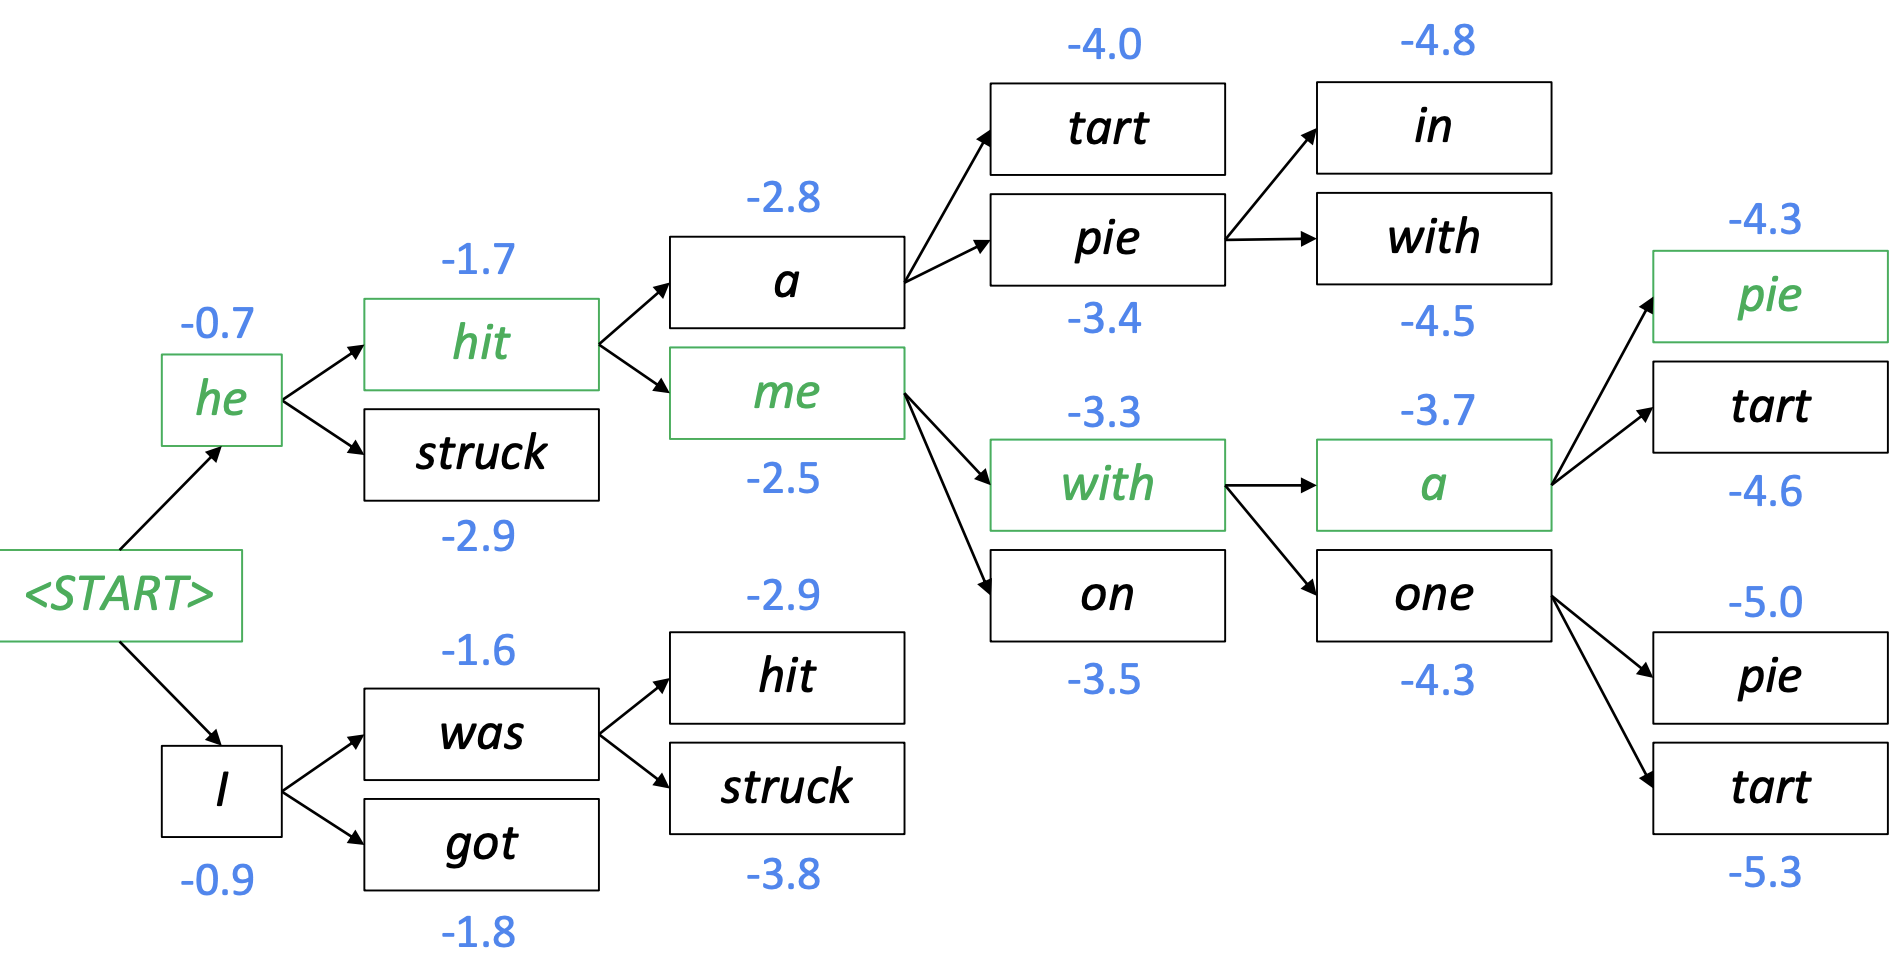
\includegraphics[height=0.6\textheight]{figures/beam-search.png}
  \end{center}
\vspace{-3mm}
\end{figure}
{\scriptsize Figure taken from \cite{stanford2019nlp}. Top-2 decoding w/ beam size 2}
\begin{itemize}
\item Keep expanding top $K>1$ hypotheses.
\item Various end conditions are possible
\begin{itemize}
\item[-] e.g. length, number of hypotheses which reached sentence end token...
\end{itemize}
\item By-product: N-best list, a list of top-N hypotheses.
\begin{itemize}
\item[-] You can check what other top hypotheses are! With that you can do e.g. model analyses, keyword detection over N-best list.
\end{itemize}
\end{itemize}
\end{frame}

%\begin{frame}{Preview, \emphbf{Exercise 8 / Assignment 4}}
%
%\begin{itemize}
%\item Final assignment.
%\item Problem which involves implementation of encoder-decoder models.
%\item Sequence to sequence models for mathematical problem solving. 
%\end{itemize}
%\end{frame}

\begin{frame}{Encoder-Decoder-Attention Models}
Back to modeling...
\begin{itemize}
\item RNNs are powerful general computers!\\ Encoder-Decoder should just work! \\(maybe separation to encoder and decoder not even needed?)
\item But practical limitation: hidden state size of RNN (memory size).
\begin{figure}
  \begin{center}
    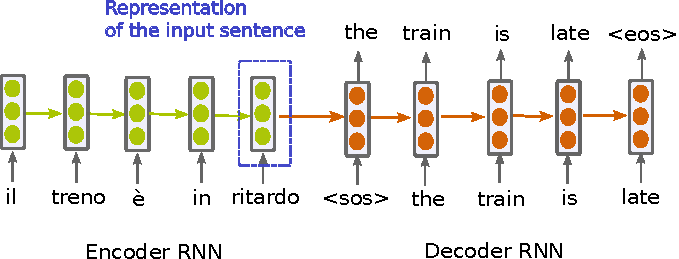
\includegraphics[height=0.3\textheight]{figures/enc-dec.pdf}
  \end{center}
\end{figure}
\pause
\item \emphbf{Attention} (Sec. 3.3) to rescue: augment decoder RNN with attention over encoder states.
\pause
\item[-] ... process the input ``piece-wise".
\item Reminder: Attention is all about key/value/query manipulation. Here queries come from the decoder,
and keys/values from the encoder.
\end{itemize}
\end{frame}

\begin{frame}{Encoder-Decoder-Attention Models,\\illustration}
The model ``focuses'' on some parts of the input (encoder states) at every decoding step.
\begin{figure}
  \begin{center}
    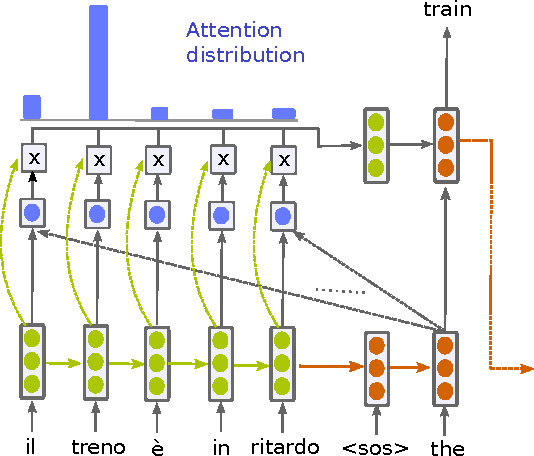
\includegraphics[height=0.9\textheight]{figures/enc-dec-att.pdf}
  \end{center}
\vspace{-3mm}
\end{figure}
\end{frame}

\begin{frame}{Modification to Encoder,\\Bi-directionality}
\begin{itemize}
\item One detail is ``sub-optimal" in the previous figure.
\item If a \textbf{standard/uni-directional} RNN is used for the encoder, the amount of information encoded in vectors at each encoder position is not equal.
\begin{itemize}
\item[-] Attention would very likely simply always focus on the vector containing the largest amounts of information.
\item[-] Encoder vector at each position should contain contexts for both past and future words.
\end{itemize}
\pause
\item Instead: we can use \emphbf{bi-directional RNNs} in the encoder.
\begin{itemize}
\item[-] Essentially 2 RNNs, reading the inputs in forward and backward directions.
\item[-] State vectors from forward and backward RNNs are \textbf{concatenated} to form the context vector for each encoder position.
\item[-] In fact, this option is part of \codeb{torch.nn.LSTM} in PyTorch \code{bidirectional=True}.
\end{itemize}
\end{itemize}
\end{frame}

\begin{frame}{Modification to Encoder,\\Bi-directionality, illustration}
\begin{figure}
  \begin{center}
    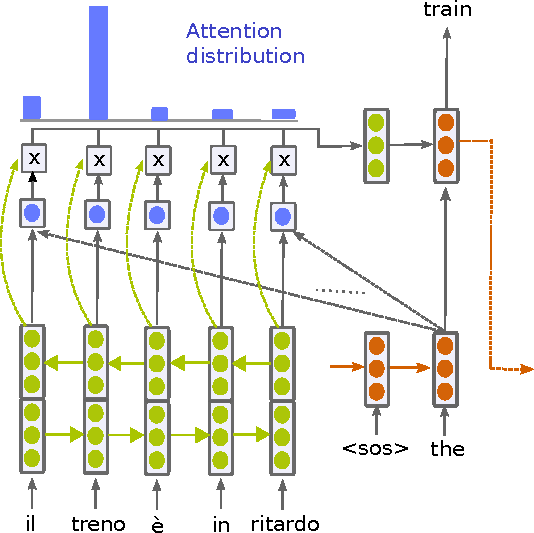
\includegraphics[height=0.9\textheight]{figures/bienc-dec-att.pdf}
  \end{center}
\vspace{-3mm}
\end{figure}
\end{frame}

\begin{frame}{Encoder-Decoder-Attention Models,\\equations}
\small{NB: there are many variants with small differences. Here, one basic variant.}\\

Given sequences of:
\begin{itemize}
\item $S$ source tokens $(x_1,..,x_S)$ with a source vocabulary $x_s \in \mathbb{S}$
\item $T$ target tokens $(y_1,..,y_T)$ with a target vocabulary $y_t \in \mathbb{T}$
\end{itemize}
Our model computes $p(y_t|y_1^{t-1}, x_1^S)$
\pause
\begin{itemize}
\item The encoder transforms $(x_1,..,x_S)$ to a \emphbf{sequence of encoder state vectors} $(h_1^{(\text{enc})},..,h_S^{(\text{enc})})$.
\item[-] Each $h_s^{(\text{enc})} = [h_s^{(\text{fwd})}, h_s^{(\text{bwd})}]_{\text{feat}} \in \mathbb{R}^{2 \times d_{\text{enc}}}$ is a concatenation of two vectors along the feature dimension.
$d_{enc}$ is the encoder RNN state dimension.
\pause
\item $h_s^{(\text{fwd})}$ and $h_s^{(\text{bwd})}$ are computed using two separate RNNs;
with two different directions, forward (fwd) and backward (bwd).
\item[-] i.e. $[h_1^{(\text{fwd})},..,h_S^{(\text{fwd})}] = \RNN_\text{fwd}(x_1^S)$ and $[h_S^{(\text{bwd})},..,h_1^{(\text{bwd})}] = \RNN_\text{bwd}(x_S^1)$ 
\end{itemize}
\pause
\vsp
Let's denote: $H^{(\text{enc})}=[h_1^{(\text{enc})}, ..., h_S^{(\text{enc})}]_{\text{time}} = \Encoder(x_1,..,x_S)$ 
\end{frame}

\begin{frame}{Encoder-Decoder-Attention Models,\\equations (cont'd)}
On the decoder side, we have the target tokens $(y_1,..,y_T)$.
\begin{itemize}
\item \emphbf{Decoder RNN state} $h_t^{(\text{dec})}$ is computed as:
\[
h_t^{(\text{dec})} = \RNNCell(h^{(\text{dec})}_{t-1}, y_{t-1}, c_t)
\]
Just like the usual RNN but with an extra dependency on $c_t$.
\pause
\item The \emphbf{context vector} $c_t$ is computed by attention (Sec. 3.3) where you use
$h^{(\text{dec})}_{t-1}$ as \textbf{query}, and $H^{(\text{enc})}$ as \textbf{key} and \textbf{value} vectors.\\
\[
c_t = \Attention(H^{(\text{enc})}, H^{(\text{enc})}, h^{(\text{dec})}_{t-1})
\]
\item The current decoder state $h_t^{(\text{dec})}$ is fed to the softmax layer to get the output $p(y_t|y_1^{t-1}, x_1^S)$.
\end{itemize}
\vsp
\pause
\scriptsize{If interested, more reading: \cite{wu2016google} \textit{Google's Neural Machine Translation System: Bridging the Gap between Human and Machine Translation}}
\end{frame}

%\begin{frame}{Can we replace RNNs by ConvNets?}
%\begin{itemize}
%\item Yes.
%\item Offers faster alternative with competitive performance on some tasks.
%\end{itemize}
%\end{frame}

\begin{frame}{Transformer models}
\small{Today's state-of-the-art model for translation.}
 \begin{minipage}{0.6\textwidth}
\vsp
\begin{itemize}
\item ``Replace" RNN layers by Transformer layers. \textit{Attention is all you need...}
\pause
\item The positional encoding is needed to both encoder and decoder inputs.
\item The decoder layers accesses the encoder states using attention.
\pause
\item Compared to what we saw in \textbf{Sec 3.3} (decoder-only/auto-regressive Transformer), this would require an \textbf{extra attention layer}. Each Transformer decoder layer consists of:
\begin{itemize}
\item[-] One self-attention layer (key/value from \emphbf{previous target tokens})
\item[-] One attention layer (key/value from \emphbf{encoder states})
\item[-] One feed-forward layer
\end{itemize}
%\vsp
%\hspace{10mm} \scriptsize{Figure taken from \cite{trafo}.}
\end{itemize}
 \end{minipage}
 \begin{minipage}{0.38\textwidth}
\begin{figure}
\vspace{-5mm}
   \begin{center}
     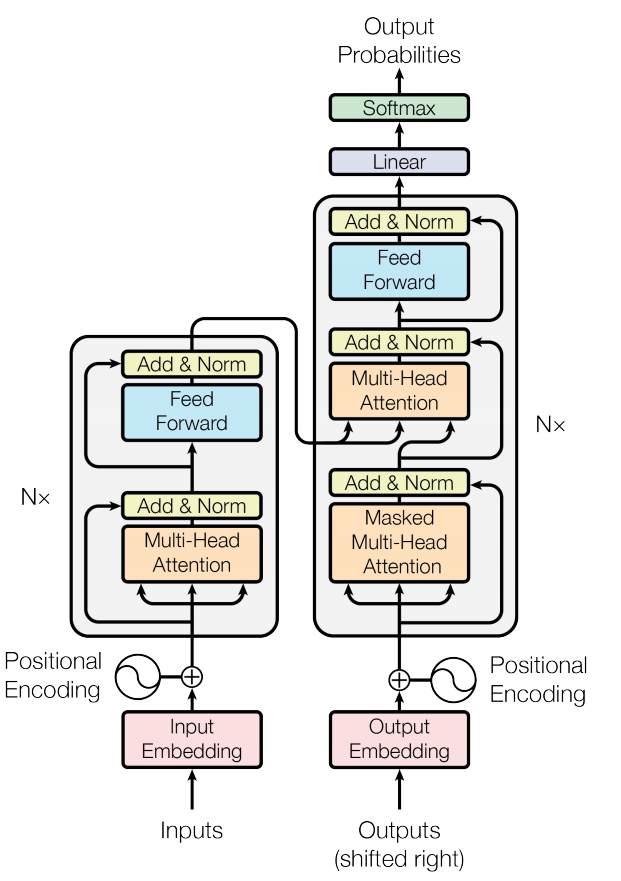
\includegraphics[width=0.9\linewidth]{figures/trafo_original.png}
   \end{center}
\end{figure}
\scriptsize{Figure from \cite{trafo}.}
 \end{minipage}
\end{frame}

\begin{frame}{Transformer models (cont'd)}
\begin{itemize}
\item All core computations are based on attention.\\
Reminder: $\Attention(K, V, Q) = V \softmax_\text{time}(K^{\intercal} Q)$
\vsp
\item The difference between the \emphbf{3 types} of attention in the Transformer are the choice of keys $K$, values $V$, and queries $Q$ used in the computation.
\vsp
\begin{itemize}
\item[-] \emphbf{Self-attention in the encoder}:\\ the whole input sequence produces all key, value and query vectors.
\vsp
\item[-] \emphbf{Decoder-to-encoder attention in the decoder}:\\ queries are decoder states, key and values are from the encoder states.
\vsp
\item[-] \emphbf{Self-attention in the decoder}:\\ query is computed from the current input to the decoder, keys and values are the previous decoder states (just like in language models)
\end{itemize}
\end{itemize}
\end{frame}


\begin{frame}{Batch and masking}
\begin{itemize}
\item \textbf{Batch}
\begin{itemize}
\item[-] Sequences with different lengths can be in the same batch.
\item[-] We need to do padding (just like before) for \emphbf{both source and target sequences}.
\item[-] Reminder: padded parts (here on the target side) should be excluded (masked) from
the computation of the loss.
\end{itemize}
\item For all attention types, the unnormalized attention weights $K^{\intercal} Q$ can be computed in a single matrix multiplication (including all positions).
\item Some positions are not valid: positions that the attention are not supposed to access can be \emphbf{masked} afterwards: ie. attention scores
of the masked positions are set to zero.
\vsp
\item \textbf{Masks for attention}
\begin{itemize}
\item[-] For each attention function, we need to specify a mask.
\item[-] The attention scores are computed for all positions in the batch.
\item[-] The parts which should not be attended should be masked, i.e. the attention score should be set to zero (or -infinity before softmax).
\end{itemize}
\end{itemize}
\end{frame}

\begin{frame}{Attention types, Illustrations}
\vspace{-5mm}
\scriptsize{Again with an example for Italian to English translation.}
\begin{figure}
% \vspace{-5mm}
   \begin{center}
     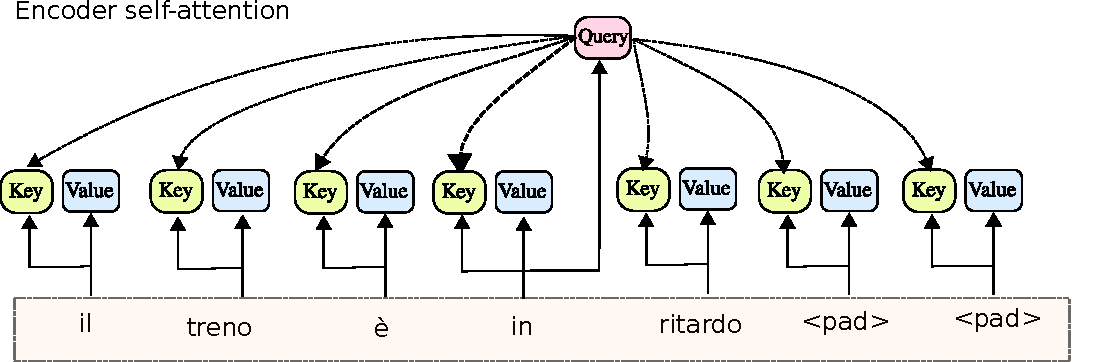
\includegraphics[width=0.7\linewidth]{figures/trafo_masks_enc_enc.pdf}
   \end{center}
\end{figure}
\vspace{5mm}
\begin{figure}
\vspace{-5mm}
   \begin{center}
     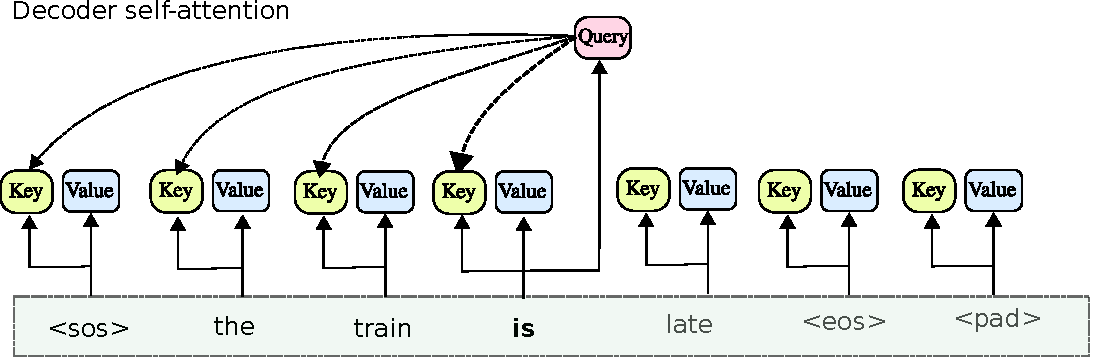
\includegraphics[width=0.7\linewidth]{figures/trafo_masks_dec_dec.pdf}
   \end{center}
\end{figure}
\end{frame}


\begin{frame}{Attention, Illustrations (cont'd)}
\begin{figure}
   \begin{center}
     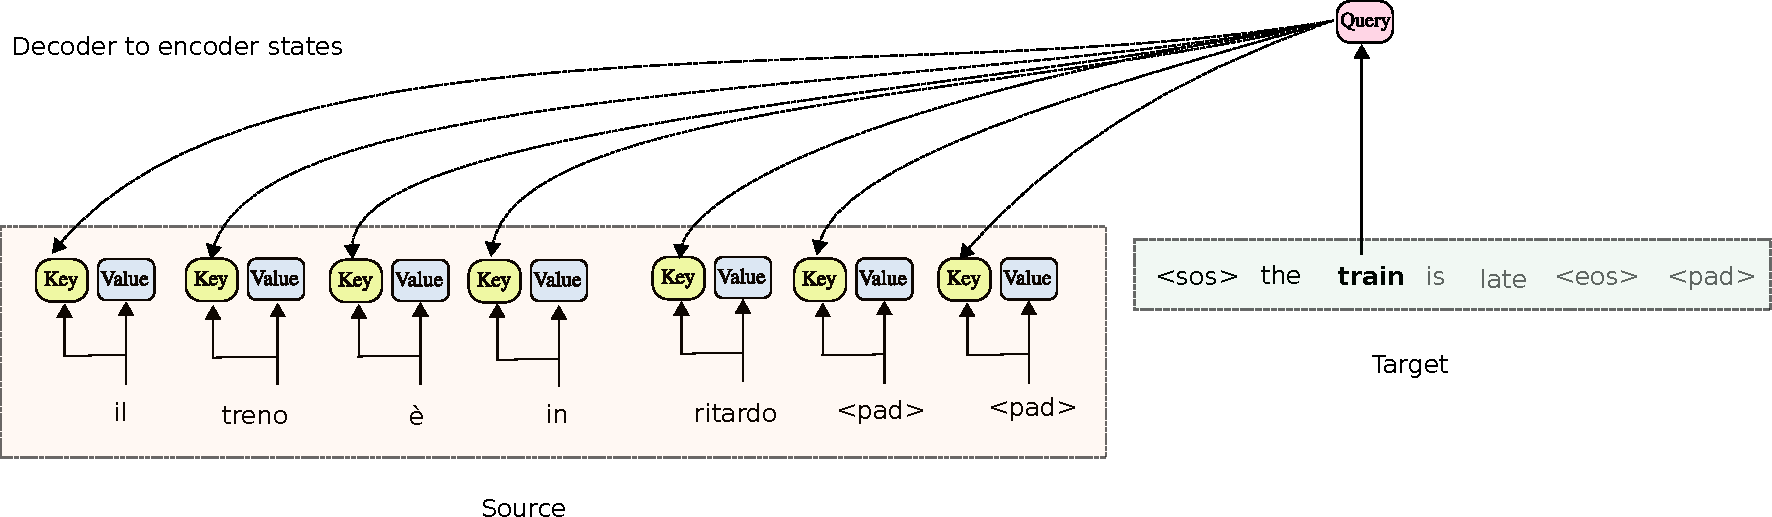
\includegraphics[width=1.0\linewidth]{figures/trafo_masks_dec_enc.pdf}
   \end{center}
\end{figure}
NB: 
\begin{itemize}
\item \texttt{<sos>} and \texttt{<eos>} are crucial for the sequence on the \emphbf{target} side
(we could also have them for the source side sequence; not illustrated here).
\end{itemize}
\end{frame}


\begin{frame}[fragile]{A few words on \code{nn.Transformer}}
\begin{itemize}
\item The official one from PyTorch, which you will use in the final assignment!
\begin{itemize}
\item[-] Maybe not the most user friendly implementation...
\item[-] Make sure to use the latest PyTorch version! ($\geq$ 1.6.0)
\end{itemize}
\item \code{nn.Transformer} implements the full \textbf{encoder-decoder model}.
\begin{itemize}
\item[-] It internally calls \code{TransformerEncoderLayer}, etc...
\item[-] Full documentation at \link{https://pytorch.org/docs/stable/generated/torch.nn.Transformer.html}
\item[-] Code: \link{https://pytorch.org/docs/stable/_modules/torch/nn/modules/transformer.html}
\item[-] The constructor is standard: you specify Transformer's hyper-parameters.
\end{itemize}
\item NB: remember we've already learned \textbf{positional encoding} in  Sec. 3.3 with an example implementation. \alert{Do not forget it!}
\item There are a couple of things you have to think, to use the forward function. 
\end{itemize}
\end{frame}

\begin{frame}[fragile]{\code{nn.Transformer}, \code{forward} (cont'd)}
% \vspace{-5mm}
There are \textbf{6 mask tensors} you can feed to the \code{forward} function.
\begin{itemize}
\item 3 \textbf{masks for padding}. You need them all (in principle):
\begin{itemize}
\item[-] \code{src\_key\_padding\_mask}
\item[-] \code{tgt\_key\_padding\_mask}
\item[-] \code{memory\_key\_padding\_mask}\\
\textbf{But} \code{memory} refers to encoder states for decoder-to-encoder attention.
So the same mask can be used for \code{src\_key\_padding\_mask} and \code{memory\_key\_padding\_mask}.
\end{itemize}
\item 3 \textbf{attention masks} for limiting the attention range:
\begin{itemize}
\item[-] \code{src\_mask}
\item[-] \code{tgt\_mask}
\item[-] \code{memory\_mask}\\
\end{itemize}
\textbf{But} only \code{tgt\_mask} has to be specified (for this assignment).
\item Method to generate \code{tgt\_mask} is implemented in \code{torch.nn.Transformer}: see \codeb{generate\_square\_subsequent\_mask}.
\item You have a choice of create masks with values: -inf/0 or True/False to specify mask/no-mask respectively (if you use the latest PyTorch version). \alert{Be careful with the meaning of True/False vs. mask/no-mask}.
\end{itemize}
%\begin{python}
%        Shape:
%            - src: :math:`(S, N, E)`.
%            - tgt: :math:`(T, N, E)`.
%            - src_mask: :math:`(S, S)`.
%            - tgt_mask: :math:`(T, T)`.
%            - memory_mask: :math:`(T, S)`.
%            - src_key_padding_mask: :math:`(N, S)`.
%            - tgt_key_padding_mask: :math:`(N, T)`.
%            - memory_key_padding_mask: :math:`(N, S)`.
%\end{python}
\end{frame}

\begin{frame}[fragile]{\code{nn.Transformer}, \code{forward} (cont'd)}

\begin{itemize}
\item \code{tgt} argument of \code{forward} function expects the \textbf{input sequence to the decoder}.
\item Reminder, it is like in language modeling: 
\begin{itemize}
\item[-] If the target side sequence is: \texttt{<sos> a b <eos>}
\item[-] The input to the decoder should be the sequence: \texttt{<sos> a b}
\item[-] While the expected output sequence (to compute the loss) is: \texttt{a b <eos>}
\end{itemize}
Make sure to correctly do the shifting!
\end{itemize}
\end{frame}


\begin{frame}[fragile]{Hints for Assignment 4, Summary}
\vspace{-5mm}
\begin{itemize}
\item Good news: Model itself is implemented in the helper code!
\item Be careful with sequences (shift) to be used in the \code{tgt} argument of \code{forward} function and the loss computation.
\item Be careful with all the \textbf{masks} for \code{forward} function.
\item Method to generate \code{tgt\_mask} is implemented in \code{torch.nn.Transformer}: \codeb{generate\_square\_subsequent\_mask}.\\ You can test it separately.
% \item Do not forget to add \textbf{positional encoding} to the source and target embedding (before you need them to Transformer layers).
\item In general, be careful with the meaning of the mask values (e.g. does 0 means mask or no-mask?)
\item To implement \textbf{greedy search}:
\begin{itemize}
\item[-] Check how the encoder and decoder submodules are called in \code{forward}.\\
\link{https://pytorch.org/docs/stable/_modules/torch/nn/modules/transformer.html}
\item[-] Remember that you can access the encoder and decoder via \code{.encoder} and \code{.decoder} once you have your Transformer object.
\end{itemize}
\end{itemize}
\end{frame}

\begin{frame}{Important announcement for\\ \emphbf{Assignment 4}}
\small
\begin{itemize}
\item The deadline is \emphbf{January 15, 2023} (Sunday at 10 pm).
\vsp
\item \textbf{Why not 2(3)-week deadline as usual?}
\item[-] To give you more time (possibility to work during the holidays if you wish).
\item[-] This does not mean that you need more than 2 weeks to solve the problem.\\
You are welcome to finish within the usual 2-week period and submit before Christmas.
% \item[-] We leave you a possibility to spend more time on this during the holidays (in case, you prefer to do so).
\vsp
\item \textbf{\alert{Warning}}:
\item[-] We know that this date is in the middle of the exam period.
\item[-] But should be better than the orignally planned date: December 24.
\item[-] There will be no extension to the deadline.
\item[-] The late submission policy will apply as usual.
\item[-] We may answer questions via email until end of December, but very likely not at all in January: Be aware of this, and ask your questions early!
\end{itemize}
\end{frame}

\begin{frame}{Important announcement for\\ \emphbf{Assignment 4} (cont'd)}
\small
\begin{itemize}
\item We will have QA sessions for A4:
\item[-] today
\item[-] next week, the second part.
\item In addition, you should not hesitate to contact us by email (even with your code).
\item Reminder: 
\item[-] Please \textbf{\alert{always}} put all TAs in CC, in any email.
\item[-] Please do not send messages via MS Chat (except during the class).
% \item[-] We leave you a possibility to spend more time on this during the holidays (in case, you prefer to do so).
\end{itemize}
\end{frame}

%\begin{frame}{Preliminaries, \emphbf{Exercise 8 / Assignment 4}}
%\begin{itemize}
%\item Mathematical problem solving as character level machine translation.
%\item Implementation of a Transformer encoder decoder model.
%\item You will use \texttt{TranslationDataset} and \texttt{Iterator} from \texttt{torchtext}.
%\item Likewise language modeling in assignment 3, tokenization needs to be done with \texttt{Field}.
%\item See hints on the previous slides.
%\end{itemize}
%\end{frame}
%
%\begin{frame}[fragile]{Preliminaries for Assignment 4,\\
%TranslationDataset/Iterator}
%\vspace{-2mm}
%\begin{python}
%
%# - TODO: Prepare `Field` object for source and target:
%#   `source_field` and `target_field`
%# - TODO: Specify path to the data: `folder`
%
%TRAIN_FILE_NAME = "train"
%VALID_FILE_NAME = "interpolate"
%
%INPUTS_FILE_ENDING = ".x"
%TARGETS_FILE_ENDING = ".y"
%
%train_dataset, valid_dataset, _ = TranslationDataset.splits(
%  path=folder,
%  root=folder,
%  exts=(INPUTS_FILE_ENDING, TARGETS_FILE_ENDING),
%  fields=(source_field, target_field),
%  train=TRAIN_FILE_NAME,
%  validation=VALID_FILE_NAME,
%  test=VALID_FILE_NAME)
%
%\end{python}
%\end{frame}
%
%\begin{frame}[fragile]{Preliminaries for Assignment 4,\\
%TranslationDataset/Iterator (cont'd)}
%\vspace{-2mm}
%\begin{python}
%# Using the generated dataset object,
%# create the iterator...
%
%train_iterator = Iterator(
%    dataset=train_dataset,
%    batch_size=train_bs,  # TODO: batch size
%    train=True,
%    repeat=False,
%    shuffle=True,
%    device=device)  # TODO: device
%
%# TODO: validation set...
%\end{python}
%\end{frame}

\begin{frame}{A generic model for any Seq2Seq tasks?}
\begin{itemize}
\item Yes.
\item Many tasks are ``translation" like.
\item Some task specific/engineering tweaks are often introduced.
\item E.g. Speech recognition: input sequence (audio) is
very long.
\item Downsampling is done using convolution or pooling in the encoder
in order to reduce the effective sequence length for RNNs/Transformers.
\end{itemize}
\end{frame}


\begin{frame}{Other tasks, e.g. image related}
\emphbf{Principle of encoding} a source information into a vector, 
and pass it to a decoder/classifier is general. Examples:
\begin{itemize}
\item Image classification: already seen!\\ convnets to encode images + classifier.
\item Image captioning
\begin{itemize}
\item Input: image $\rightarrow$ encode it with convnets.
\item Output: text describing image $\rightarrow$ generate it with RNNs or Transformers.
\end{itemize}
\item Image question answering
\begin{itemize}
\item Inputs: image and text/question.
\item Output: text or just answer token.
\end{itemize}
\end{itemize}
Again, some task specific models are designed for the best
performance, but the idea of encoding/decoding
is general.\\
Encoders learn compact representations of inputs.
\end{frame}

%\begin{frame}{Encoder, Decoder}
%Many tasks: some encoding and decoding of different
%modalities. connecting them together.
%Image captionig:
%input: image -> convolution
%
%
%Before: needed to hand crafted features.
%Now: end-to-end differentiable function.
%\end{frame}

%
%\begin{frame}{Sequence processing, different problem types}
%On the problem level:
%\begin{itemize}
%\item Many to one: e.g. text classification.
%\item Many to many: e.g. machine translation.
%\item One to many: some decompression tasks (?).
%\end{itemize}
%\vsp
%\textbf{Note}: Many problems fall into these sequence processing tasks (not only natural language related).\\
%\vsp
%RNNs are relevant for any of these tasks.\\
%\textbf{More important distinction for sequence processing:}
%\begin{itemize}
%\item Sequences are targets: need to be predicted/generated.
%\item Full sequence is available as source for prediction.
%e.g. text classification.
%\end{itemize}
%\end{frame}

\begin{frame}{Summary}
\textbf{What have we learned?}
\begin{itemize}
\item Building models
\item Examples of end-to-end differentiable models.
\item Encoders, decoders
\item Sequence-to-sequence problems and beyond.
\end{itemize}
\vsp
\textbf{Coming up next...}
\begin{itemize}
\item More on practical aspects for training (Chapter 5).
\item ...
\end{itemize}
\end{frame}
